\section{Zielsetzung}
In diesem Versuch soll mit einem Michelson-Interferometer
die Wellenlänge eines Lasers sowie den Brechungsindex von Luft
ermittelt werden.
\section{Theorie}
\subsection{Begriff der Interferenz}
Da es unteranderem bei dem Michelson-Interferometer um Interferenzen geht,
wird der Begriff zunächst näher erläutert.
Licht ist eine elektromagnetische Wellen und mithilfe der Maxwellschen Gleichungen
lässt sich die elektrische Feldstärke $\vec{E}$ darstellen als
\begin{equation*}
  \vec{E}(x,t) = \vec{E}_0 cos(kx-\omega t - \delta).
\end{equation*}
Dabei ist $k = \frac{2\pi}{\lambda}$ die Wellenzahl mit $\lambda$ als Wellenlänge, $\omega$ die Kreisfrequenz
und $\delta$ ein beliebiger Phasenwinkel. Für solche Gleichungen gilt das Superpositionsprinzip.
Das Prinzip sagt aus, dass in einem Raumpunkt $P$ mehrere Lichtwellen überlagern können. Da es keine Möglichkeit gibt,
solche Lichtwellen zu messen, werden lediglich die Intensitäten $I$ gemessen. Es gilt folgender Zusammenhang
\begin{equation*}
  I = const |\vec{E}|^2
\end{equation*}
Eine Addition zweier Intensitäten von Lichtwellen ergibt sich somit zu
\begin{equation*}
  I_{1+2} = 2const\vec{E}^2_0 (1+cos(\delta_2 - \delta_1)).
\end{equation*}
Der zweite Summand bildet den \textbf{Interferenzterm} und ist abhängig von der Phase $(\delta_2 - \delta_1)$
der einzelnen Wellen. Zu erkennen ist, dass bei ungerades Vielfaches von $\pi$ der Term verschwindet und somit destruktive
Interferenzen auftreten.
\subsection{Begriff der Kohärenz}
In diesem Teil wird noch die Kohärenz näher erläutert. Aus Erfahrung treten bei zwei unabhängigen Lichtquellen
keine Interferenzeffekte auf. Dies liegt daran, da die Phasenkonstanten $\delta_1$ und $\delta_2$ eine Mittlung über einen
Zeitraum der größer als die Periodendauer ist verschwinden. Die Ursache liegt im Entstehungsmechanimus des Lichtes.
Wenn ein angeregtes Atom in ihren Grundzustand zurückgehen, wird Energie in Form von elektromagnetischen Wellen abgegeben.
Die Wellen besitzen dabei eine \textbf{endliche} Länge. Wird nun über die Zeit statistisch gemittelt, verschwindet der Interferenzterm und
das Licht wird als \textbf{inkohärent} bezeichnet.
Für ein Kohörentes Licht muss daher die Wellenzahl $k$, Kreisfrequenz $\omega$ und Phasenwinkel $\delta$ konstant sein.
Dies wird zum Beispiel mit einem \textbf{LASER}(=light amplification by stimulated emission of radiation) möglich gemacht.
\subsection{Das Michelson-Interferometer}
Bei dem Michelson-Interferometer wird ein Lichtstrahl in zwei Teilstrahlen aufgeteilt. Eine schematische Darstellung
ist in Abbildung \ref{abb:1} dargestellt.
\begin{figure}[H]
  \centering
  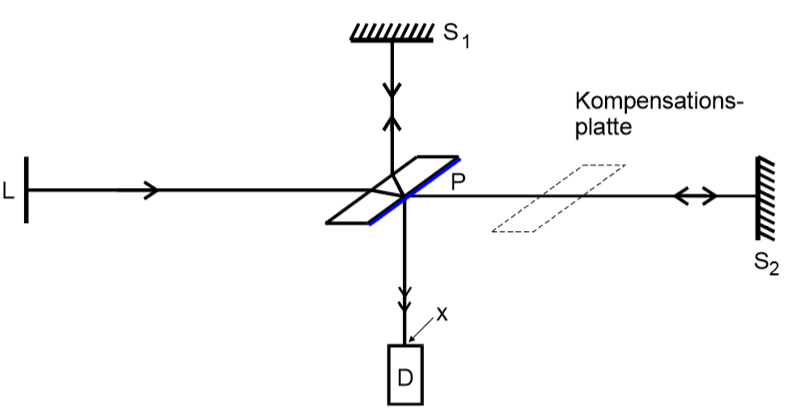
\includegraphics[width=\textwidth]{content/Aufbau.png}
  \caption{Schematische Darstellung des Michelson-Interferometers.\cite{1}}
  \label{abb:1}
\end{figure}
Im Zentrum befindet sich ein Fresnelschen Biprisma. Es lässt ein Teil des Strahls
durchgehen während ein anderer Teil eine senkrechte Änderung der Richtung erfährt. Dabei sind
$S_1$ und $S_2$ Spiegel, die den Teilstrahl zurück zum Prisma reflektieren.
Am Prisma werden sie erneut geteilt und am Detektor $D$ aufgenommen.
Wichtig für die Messung ist, dass am Detektor $D$ Interferenzen zu sehen sind.
Dies wird möglich gemacht,
wenn die Streckenabstände zu den beiden Spiegeln gleich sind und zur Strecke zum Spiegel $S_2$ eine
Kompensationsplatte liegt. Die Kompensationsplatte muss da liegen, da der Strahl von $S_2$ einmal durchs
Prisma geht, während der von $S_1$ kommende Strahl dreimal durchs Prisma geht. Der Gangunterschied
muss fast gleich sein, da die Strahlenbündel sonst nicht kohärent wären.
Da Lichtstrahlen eine endliche Länge besitzen, gibt es eine so genannte Kohärenzlänge, welche den maximalen Wegunterschied
beschreibt bei dem noch Interferenzen auftreten können.
Nun lässt sich am Detektor $D$ einen Gangunterschied von $\frac{\lambda}{2}$ feststellen.
Die dort auftreffenden Strahlen löschen sich aus. Wird nun ein Spiegel um $\Delta d$ verschoben,
so ändert sich die Intensität am Detektor $D$. Nun werden die auftretenden Helligkeitsmaxima abgezählt.
Es gilt daher folgender Zusammenhang zwischen Verschiebung des Spiegels und der Überlagerung der Strahlen
\begin{equation}
  \Delta d = z \frac{\lambda}{2}.
  \label{eq:1}
\end{equation}
Dabei ist z die Anzahl der auftretenden Helligkeitsmaxima.
Eine weitere Möglichkeit um Interferenz zu erzeugen ist, dass sie durch ein Medium mit der Länge $b$ mit
einem geändertem Brechungsindex $n+\Delta n$ durchlaufen.
Eine schematische Darstellung ist in Abbildung \ref{abb:2} zu sehen.
\begin{figure}[H]
  \centering
  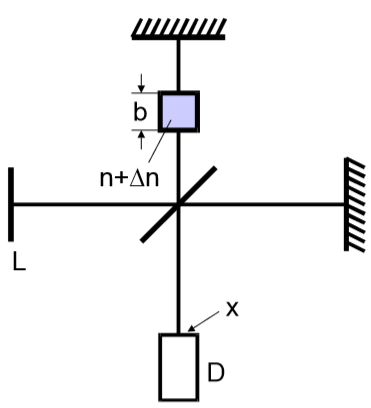
\includegraphics[width=0.5\textwidth]{content/Aufbau2.png}
  \caption{Weitere Darstellung des Michelson-Interferometers zur Bestimmung des Brechungsindex.\cite{1}}
  \label{abb:2}
\end{figure}
$n$ beschreibt dabei an allen anderen Orten den Brechungsindex den Wert $n$. Der optische
Wegunterschied beträgt nun $b\Delta n$.
Durch evakuieren der Messzelle oder durch erhöhen des Drucks in der Messzelle, kann der Detektor $d$
wieder Helligkeitsmaxima zählen, da sich der Brechungsindex und somit der optische
Wegunterschied ständig ändert. Es gilt nun folgender Zusammenhang
\begin{equation}
  b\Delta n = z \frac{\lambda}{2}
  \label{eq:2}
\end{equation}
Aus der klassischen Dispersionstheorie lässt sich zwischen dem Brechungsindex $n$ und
der Zahl $N$, welche die von den Lichtwellen erzwungenen Schwingungen pro Volumeneinheit ist, durch Näherung folgender
Zusammenhang schreiben:
\begin{equation*}
  n = 1+\frac{f(\lambda)}{2}N
\end{equation*}
Voraussetzung ist das Luft im Bereich von $0$ bis $1$ Bar sich als ideales Gas verhält.
Daraus folgt das die Anzahl der Moleküle $N$ gegeben ist durch
\begin{equation*}
  N = \frac{p}{T} \frac{T_0}{p_0} N_L
\end{equation*}
Dabei ist $N_L$ die Loschmidtsche Zahl, $p$ der Druck beziehungsweise $p_0$ der Umgebungsdruck und
$T$ die Temperatur.
Für eine Änderung des Brechungsindex kann nun folgende Gleichung angewendet werden
\begin{equation*}
  \Delta n = \frac{f}{2} N_L \frac{T_0}{p_0}\frac{1}{T} (p-p').
\end{equation*}
Dabei ist $p-p'=\Delta p$ die Druckdifferenz der Platte.
Nun soll die klassische Dispersionstheorie erfüllt werden und somit gilt dann
\begin{equation*}
  n = 1 + \Delta n \frac{T}{T_0} \frac{p_0}{\Delta p}
\end{equation*}
Mit der Gleichung \ref{eq:2} kann folgender Zusammenhang zwischen Druck und Brechungsindex
hergeleitet werden. Dazu wird aus Gleichung \ref{eq:2} nach $\Delta n$ umgeformt und
in die vorherige Gleichung eingesetzt. Es folgt
\begin{equation}
  n = 1 + \frac{z \lambda}{2b} \frac{T}{T_0} \frac{p_0}{\Delta p}.
  \label{eq:3}
\end{equation}
Dabei verhält sich die Temperatur $\frac{T}{T_0} \approx 1$.
